\chapter{Means Comparison}\label{ch:mc}

\section{Methods}

\subsection{Introduction}
Bull run and Kingston power plants installed scrubbers in the year 2008 as mandated by the EPA.
These scrubbers may have significantly reduced the amount of sulfur dioxide emitted by the smoke stacks.
According to \autoref{fig:sulfateemissions}, which is a bar chart depicting the sum of sulfur dioxide emissions of Kingston and Bull run power plants,  the sulfur dioxide concentration dropped from 80 thousand tons in 2008 to about 15 thousand tons in 2009.
Interestingly the through fall SO$_4$ concentrations dramatically decline from about 115 $\mu$eq L$^{-1}$ in 2007 to about 30 $\mu$eq L$^{-1}$ in 2010.
\begin{figure}[h!]
  \centering
  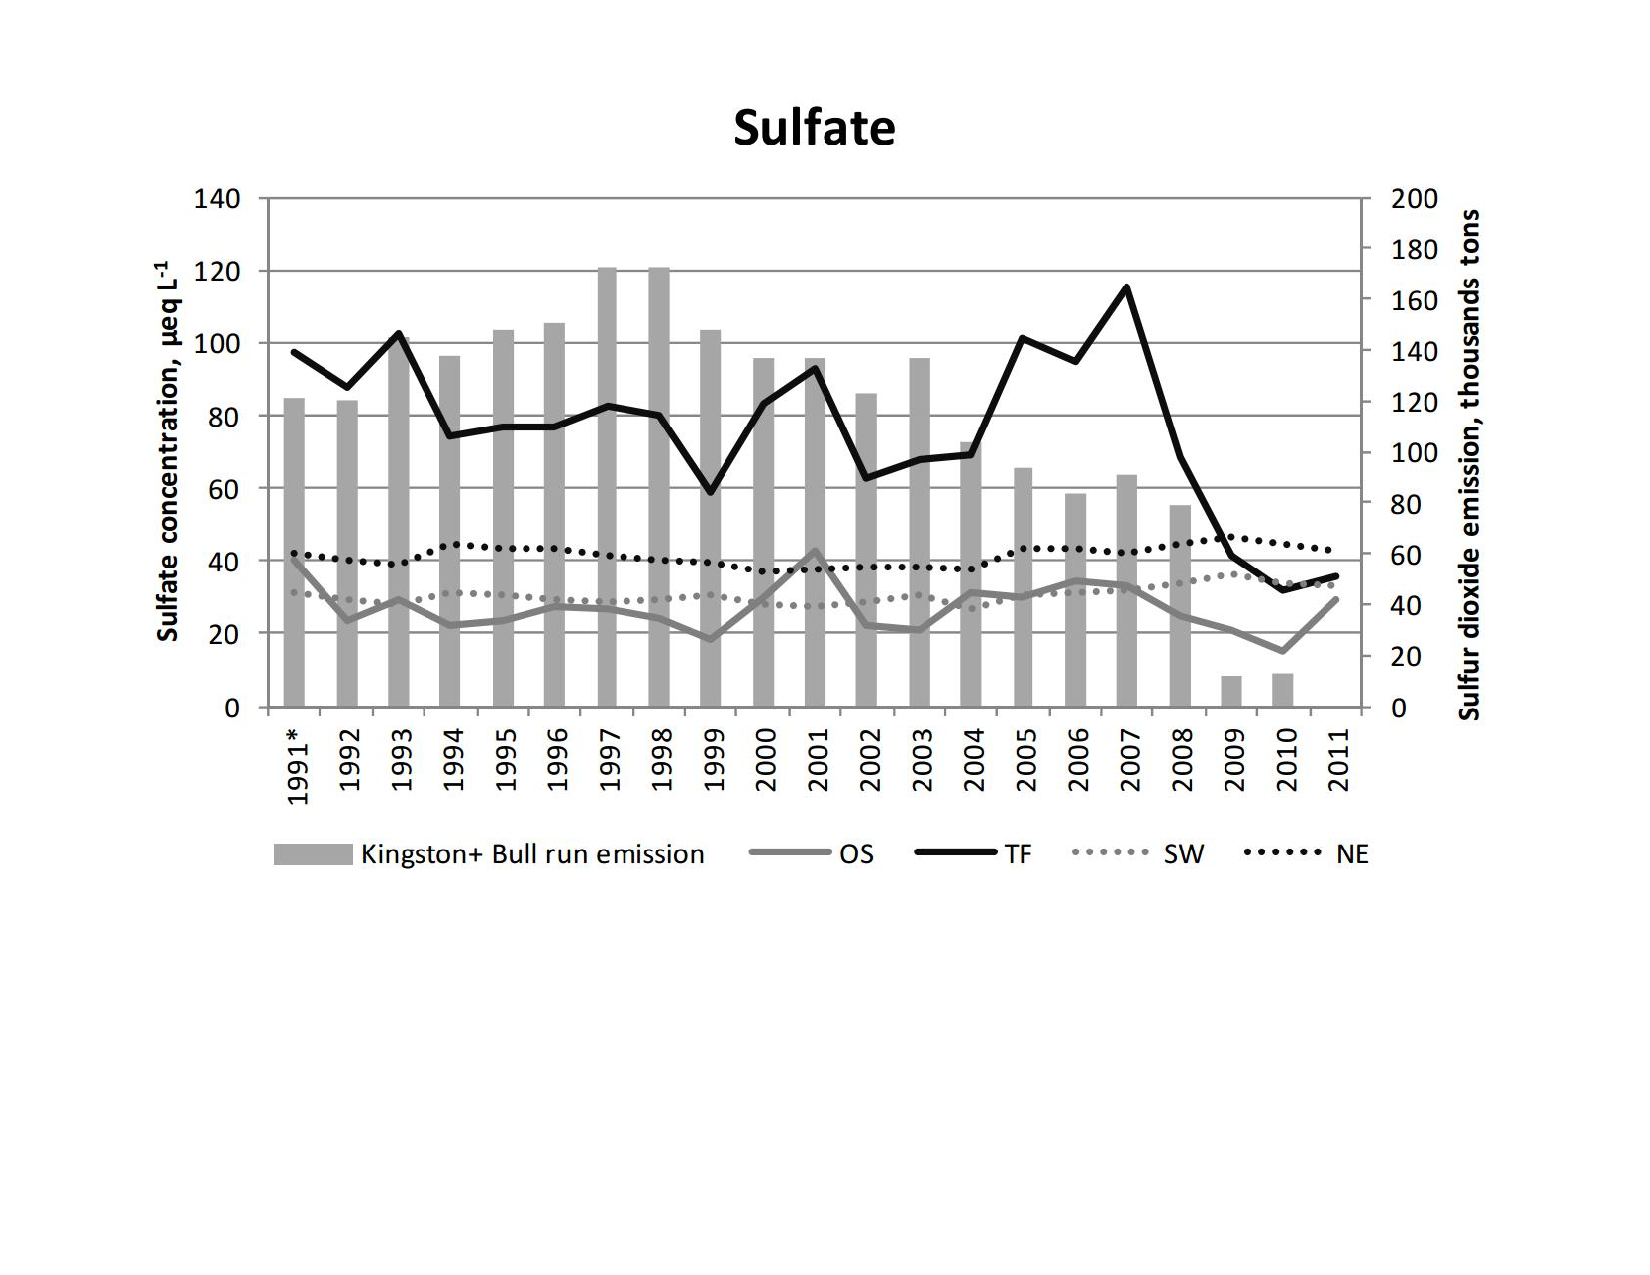
\includegraphics[width=6in]{SulfateEmissions}\\
  \caption{Sulfate emmisions of Kingstion and Bull run against those measured in Noland high elevation site \citep{annualreport2012}.}\label{fig:sulfateemissions}
\end{figure}
The hypothesis is that the decrease in sulfur dioxide emissions could correlate to the decrease in SO$_4$ concentrations measured in Noland Divide through fall.
And assuming that the sulfur dioxide emissions from Kingston and Bull run power plants affect the whole GRSM park then there may be signals for this affect in the data.
To examine this each time set will be tested against each other by way of means comparison methods.

\subsubsection{Instruments}
ANOVA is the standard means comparison method.
But it cannot compare more than two groups at once , and a method is needed that can compare all three time sets.
The Bonferroni multiple comparisons method is an option in the SPSS statistical program and can compare more than two groups at a time.
The explanation of the Bonferroni method given by the SPSS manual is that this method uses t tests to perform pairwise comparisons between group means and that the observed significance level is adjusted for the fact that multiple comparisons are being made \citep{spss}.

The Bonferroni method will create two specific types of outputs.
The first is a line graph showing the means of each group analyzed.
And the second is  a table of pairwise listings of all the groups compared to each other.
This table contains 95$\%$ confidence intervals and the significance associated with each comparison.
These confidence intervals are produced by the difference in means between the two groups being compared.
If the confidence interval includes zero then the groups are statistically the same or equal.

Using SPSS and the Bonferroni method three time sets (93-02, 03-08, 09-12) will be compared at six elevation class levels and across four water quality variables (pH, ANC, NO$_3$, and SO$_4 $).
Each group compared is the same stream survey data analyzed in chapter 2 and chapter 4 of this paper.

\section{Results}
\begin{table}[htbp]
\caption{Bonferroni comparisons between multiple groups}
\begin{center}
\begin{tabular}{p{2cm}cccccccccccc}
\toprule
 Elevation Classes& \multicolumn{ 3}{c}{pH} & \multicolumn{ 3}{c}{ANC} & \multicolumn{ 3}{c}{Nitrate} & \multicolumn{ 3}{c}{Sulfate} \\ \cline{2-13}\noalign{\smallskip}
 & \multicolumn{ 1}{c}{1-2} & 1-3 & 2-3 & 1-2 & 1-3 & 2-3 & 1-2 & 1-3 & 2-3 & 1-2 & 1-3 & 2-3 \\  \cline{2-13}
\multicolumn{1}{c}{1} & \textbf{$\neq$} & \textbf{$\neq$} & \textbf{$\neq$} & \textbf{=} & \textbf{=} & \textbf{=} & \textbf{$\neq$} & \textbf{=} & \textbf{=} & \textbf{=} & \textbf{=} & \textbf{=} \\ 
\multicolumn{1}{c}{2} & \textbf{=} & \textbf{=} & \textbf{=} & \textbf{=} & \textbf{$\neq$} & \textbf{=} & \textbf{$\neq$} & \textbf{$\neq$} & \textbf{=} & \textbf{$\neq$} & \textbf{$\neq$} & \textbf{=} \\ 
\multicolumn{1}{c}{3} & \textbf{$\neq$} & \textbf{$\neq$} & \textbf{$\neq$} & \textbf{=} & \textbf{$\neq$} & \textbf{=} & \textbf{=} & \textbf{$\neq$} & \textbf{$\neq$} & \textbf{=} & \textbf{=} & \textbf{=} \\ 
\multicolumn{1}{c}{4} & \textbf{=} & \textbf{$\neq$} & \textbf{$\neq$} & \textbf{=} & \textbf{=} & \textbf{=} & \textbf{=} & \textbf{=} & \textbf{=} & \textbf{=} & \textbf{=} & \textbf{=} \\ 
\multicolumn{1}{c}{5} & \textbf{$\neq$} & \textbf{$\neq$} & \textbf{$\neq$} & \textbf{=} & \textbf{$\neq$} & \textbf{$\neq$} & \textbf{$\neq$} & \textbf{=} & \textbf{$\neq$} & \textbf{=} & \textbf{=} & \textbf{=} \\ 
\multicolumn{1}{c}{6} & \textbf{=} & \textbf{$\neq$} & \textbf{$\neq$} & \textbf{=} & \textbf{=} & \textbf{=} & \textbf{=} & \textbf{=} & \textbf{=} & \textbf{=} & \textbf{=} & \textbf{=} \\ 
\bottomrule
\end{tabular}
\end{center}
\label{tab:Bontable}
\end{table}
\autoref{tab:Bontable} reports the Bonferoni comparison means between the four water quality variables (pH, ANC, NO$_3$, SO$_4$) in one time set against the same water quality variable in another time set by elevation bands.
In the table there are three columns per water quality variable.
And each column represents the comparison of two groups of the same variable in different times.
If the Bonferroni comparison found the groups to be equal then equality was represented by an equal sign.
If the groups are not equal an not equal sign was used to show this.
%state significance as all equals are significant, look at the data. open output through spss
All groups that are equal are also insignificant and all groups that are unequal are significant at a starting $ \alpha$ of .05.

The set comparisons between pH are the first comparisons presented.  
Mostly all the sets are different except between elevation class 2 which is all the same and class 4 and 6 which show sets 1 and 2 being equal.  
The next variable is ANC.  
The comparison found a lot of equality between the means of the ANC sets.  
Elevations 1, 4, and 6 are all equal.  
At elevations 2 and 3 set 1 and 3 are the only sets that are unequal. 
And at elevation 5 sets 1 and 2 are equal but set 3 is not.
For NO$_3$ elevation classes 4 and 6 are all the same and elevation 3 shows sets 1 and 2 being equal where 3 is not.  
Elevation class 1 is the opposite of expected showing all being equal except for sets 1 and 2.  
In elevation class 2 sets 3 and 2 are equal and in elevation class 5 sets 3 and 1 are equal.
SO$_4$ shows all three sets being equal across all elevation classes except for class 2.  
Class 2 shows only sets three and two being equal.

%results across sets
%results by comparison to trends

The bonferoni figures are presented in \autoref{app:bon}.
There are six figures for each of the water quality variables, one for each of the elevation classes.
These figures can sometimes be misleading when visually comparing groups and it is always best to have the confidence intervals on hand.
% an example of misleading figures
%anc has a negative trend
%results by comparison to trends

\section{Discussion}
\begin{itemize}
	\item Are these results a special case?
	\item Do these differences show up in other water quality analyses, not in the S.S.?
	\item What are the reasons that the means are higher or lower than expected?
	\item Differences between sets 2 and 3 were expected due to the scrubbers, did this occur?
	\item Why aren't the results as clear as the chart in the \citep{cai2012}?
	\begin{itemize}
		\item probably math
	\end{itemize}
	\item General hypothosis about what the results suggest
	\begin{itemize}
		\item The results suggest that a larger difference is needed to see a sulfate difference between sets 2 and 3.
	\end{itemize}
\end{itemize}